\documentclass[a4paper]{article}
\addtolength{\hoffset}{-2.25cm}
\addtolength{\textwidth}{4.5cm}
\addtolength{\voffset}{-3.25cm}
\addtolength{\textheight}{5cm}
\setlength{\parindent}{15pt}

\usepackage[unicode=true, colorlinks=false, hidelinks]{hyperref}
\usepackage[utf8]{inputenc}
\usepackage[english, russian]{babel}
\usepackage{mathtext}
\usepackage[T2A, TS1]{fontenc}
\usepackage{microtype} % Slightly tweak font spacing for aesthetics
\usepackage{amsthm, amssymb, amsmath, amsfonts, nccmath}
\usepackage{nicefrac}
\usepackage{epstopdf}
\usepackage[export]{adjustbox}
\usepackage{float} % Improved interface for floating objects
\usepackage{graphicx, multicol} % Enhanced support for graphics
\usepackage{pdfrender,xcolor}
\usepackage{breqn}
\usepackage{mathtools}
\usepackage{titling}
\usepackage{bm}
\usepackage{centernot}
\usepackage[cal=boondoxo,calscaled=.96]{mathalpha}
\usepackage{marvosym, wasysym} % More symbols
\usepackage{rotating} % Rotation tools
\usepackage{censor} % Facilities for controlling restricted text

\usepackage{fancyhdr}
\pagestyle{fancy}
\fancyhead{}\renewcommand{\headrulewidth}{0pt}
\fancyfoot[L]{}
\fancyhead{}
\fancyfoot{}
\fancyfoot[R]{\thepage}
\begin{document}
\begin{titlepage}
   \begin{center}
       \vspace*{3cm}
       \large{САНКТ-ПЕТЕРБУРГСКИЙ ПОЛИТЕХНИЧЕСКИЙ УНИВЕРСИТЕТ}
       \vspace{0.4 cm}
       
       \large\textbf{Институт прикладной математики и механики}
       \vspace{0.4 cm}
       
       \large{Высшая школа прикладной математики и вычислительной физики}
       
       \vspace{3 cm}
       \normalsize\textbf{Отчет\\ по лабораторным работам №1-2 \\ по дисциплине \\ <<Математическая статистика>>}
       \vfill
       \begin{flushright}
            \normalsize{Выполнил студент:\\
            Козлов Борис\\
            группа: 3630102/80301}
            \vskip\medskipamount
            \normalsize{Проверил:
            
            к.ф.-м.н., доцент\\
            Баженов Александр Николаевич
            }
       \end{flushright}
            
       \vspace{0.8cm}
     
            
       \normalsize{Санкт-Петербург\\2021 г.}
            
   \end{center}
\end{titlepage}
\tableofcontents
\addtocontents{toc}{~\hfill\textbf{Страница}\par}
\newpage
\listoffigures
\addtocontents{lof}{~\hfill\textbf{Страница}\par}
\newpage
\listoftables
\addtocontents{lot}{~\hfill\textbf{Страница}\par}
\newpage
\section{Постановка задачи}
Для 5 распределений:
\begin{itemize}
    \item Нормальное распределение $N(x, 0, 1)$
    \item Распределение Коши $C(x, 0, 1)$
    \item Распределение Лапласа $L(x, 0, \frac{1}{\sqrt{2}})$
    \item Распределение Пуассона $P(k, 10)$
    \item Равномерное распределение $U(x,-\sqrt{3},\sqrt{3})$
\end{itemize}
\begin{enumerate}
    \item Сгенерировать выборки размером 10, 50 и 1000 элементов. Построить на одном рисунке гистограмму и график плотности распределения.
    \item Сгенерировать выборки размером 10, 100 и 1000 элементов.
    Для каждой выборки вычислить следующие статистические характеристики положения данных: $\overline{x}, med\,x, z_R, z_Q, z_{tr}$. Повторить такие вычисления 1000 раз для каждой выборки и найти среднее характеристик положения и их квадратов:
    \begin{equation}\label{mean_formula}
        E(z)=\overline{z}
    \end{equation}
    Вычислить оценку дисперсии по формуле:
    \begin{equation}\label{variance_formula}
        D(z)=\overline{z^2}-\overline{z}^2
    \end{equation}
    Представить полученные данные в виде таблиц.
\end{enumerate}
\section{Теория}
\subsection{Рассматриваемые распределения}
Плотности:
\begin{itemize}
    \item Нормальное распределение
    \begin{equation}\label{norm}
        N(x,0,1)=\frac{1}{\sqrt{2\pi}}e^{-\frac{x^2}{2}}
    \end{equation}
    \item Распределение Коши
    \begin{equation}\label{cauchy}
        C(x, 0, 1)=\frac{1}{\pi}\frac{1}{x^2+1}
    \end{equation}
    \item Распределение Лапласа
    \begin{equation}\label{laplace}
        L(x,0,\frac{1}{\sqrt{2}})=\frac{1}{\sqrt{2}}e^{-\sqrt{2}|x|}
    \end{equation}
    \item Распределение Пуассона
    \begin{equation}\label{poisson}
        P(k, 10)=\frac{10^k}{k!}e^{-10}
    \end{equation}
    \item Равномерное распределение
    \begin{equation}\label{uniform}
        U(x,-\sqrt{3},\sqrt{3})=
        \begin{cases}
        \displaystyle\frac{1}{2\sqrt{3}}&\text{при}\;\;|x|\:\leq\sqrt{3}\\
        \;\;\;0&\text{при}\;\;|x|\:>\sqrt{3}\\
        \end{cases}
    \end{equation}
\end{itemize}
\subsection{Гистограмма}
\subsubsection{Построение гистограммы}
Множество значений, которое может принимать элемент выборки, разбивается на несколько одинаковых интервалов, откладываемых на горизонтальной оси, над каждым из которых затем рисуется прямоугольник. Высота каждого прямоугольника пропорциональна числу элементов выборки, попадающих в соответствующий интервал. 
\subsection{Вариационный ряд}
Последовательность $\displaystyle\{x_{(k)}\}_{k=1}^n$ элементов выборки размера $n$, расположенных в неубывающем порядке, называется вариационным рядом.
\subsection{Выборочные числовые характеристики}
\subsubsection{Характеристики положения}
\begin{itemize}
    \item Выборочное среднее
    \begin{equation}\label{mean}
        \overline{x}=\frac{1}{n}\sum_{i=1}^n x_i
    \end{equation}
    \item Выборочная медиана
    \begin{equation}\label{med}
        med\,x = \begin{cases}
        \displaystyle\;\;\;\;\;x_{(l+1)}&\text{при}\;\;n=2l+1\\
        \displaystyle\frac{x_{(l)}+x_{(l+1)}}{2}&\text{при}\;\;n=2l
        \end{cases}
    \end{equation}
    \item Полусумма экстремальных выборочных элементов
    \begin{equation}\label{exhfsum}
        z_R=\frac{x_{(1)}+x_{(n)}}{2}
    \end{equation}
    \item Полусумма квартилей\\
    Выборочный квартиль $z_p$ порядка $p$ определяется формулой
    \begin{equation}
        z_p = \begin{cases}\label{pqv}
        \displaystyle\;\;x_{([np]+1)}&\text{при}\;\;np\;\text{дробном,}\\
        \displaystyle\;\;\;\;\;x_{(np)}&\text{при}\;\;np\;\text{целом}
        \end{cases}
    \end{equation}
    Полусумма квартилей
    \begin{equation}\label{hfsum}
        z_Q=\frac{z_{1/4}+z_{3/4}}{2}
    \end{equation}
    \item Усечённое среднее
    \begin{equation}\label{trmean}
        z_{tr}=\frac{1}{n-2r}\sum_{i=r+1}^{n-r}x_{(i)},\;\;r\approx\frac{n}{4}
    \end{equation}
\end{itemize}
\subsubsection{Характеристики рассеивания}
Выборочная дисперсия
\begin{equation}\label{svar}
    D=\frac{1}{n}\sum_{i=1}^n \left(x_i-\overline{x}\right)^2
\end{equation}
\section{Реализация}
Лабораторная работа выполнена на языке Python в средах PyCharm и Jupyter Notebook с использованием следующих библиотек:
\begin{enumerate}
    \item scipay (генерация выборок)
    \item matplotlib, seaborn (визуализация, построение гистограмм)
    \item numpy (вычисление ряда числовых характеристик)
\end{enumerate}
\section{Результаты}
\subsection{Гистограммы и графики плотности распределения}
\begin{figure}[H]
    \centering
    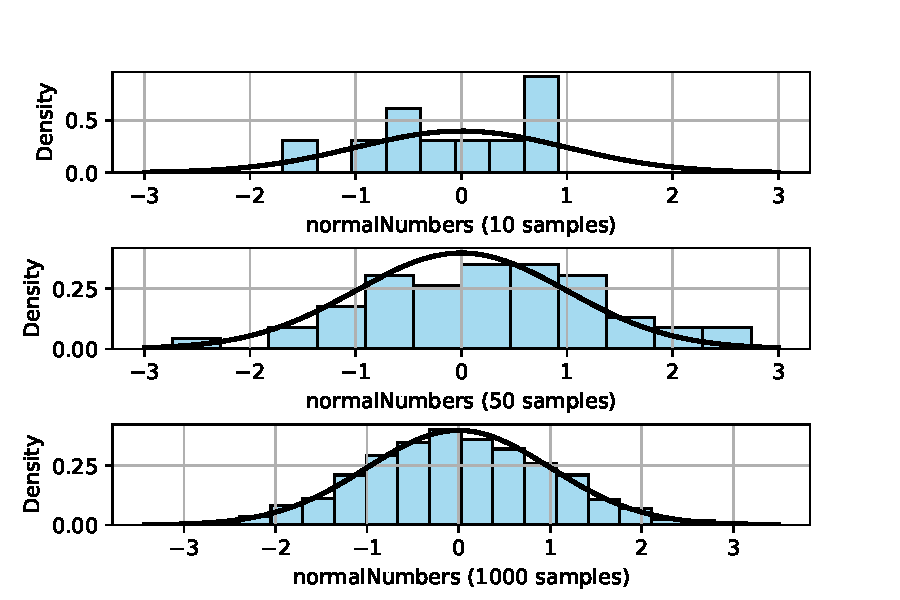
\includegraphics[width = 16 cm]{sources/normalNumbers.pdf}
    \caption{Нормальное распределение \eqref{norm}}
    \label{fig:norm}
\end{figure}
\begin{figure}[H]
    \centering
    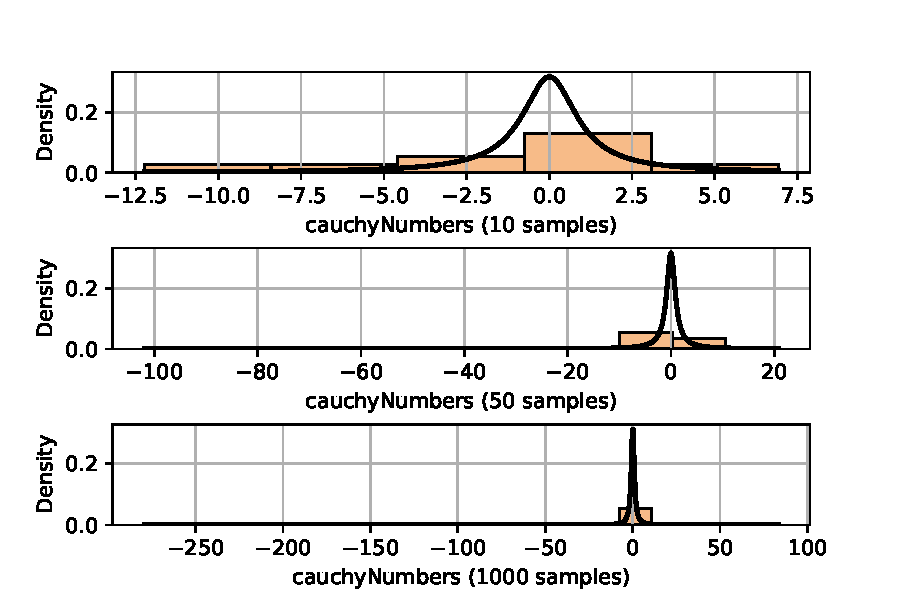
\includegraphics[width = 16 cm]{sources/cauchyNumbers.pdf}
    \caption{Распределение Коши \eqref{cauchy}}
    \label{fig:cauchy}
\end{figure}
\begin{figure}[H]
    \centering
    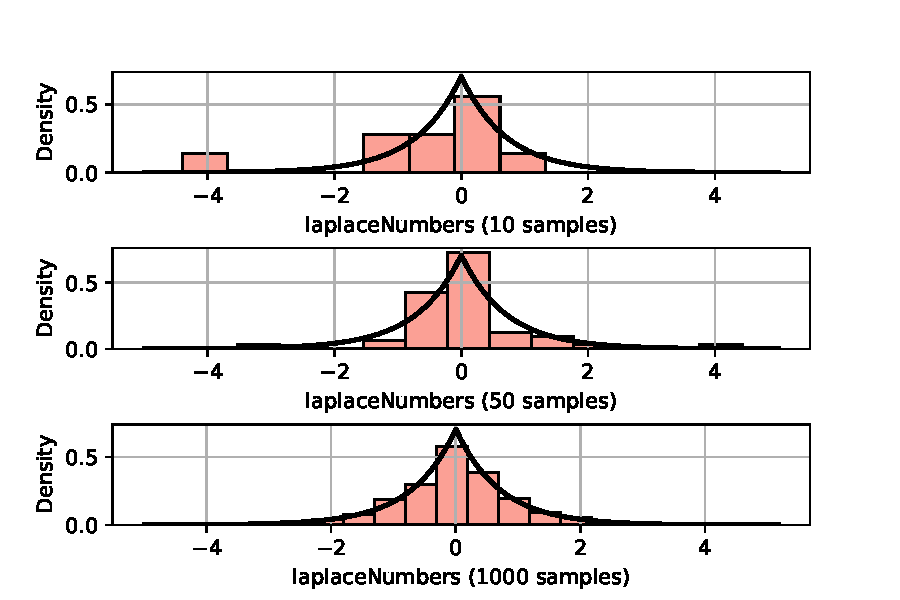
\includegraphics[width = 16 cm]{sources/laplaceNumbers.pdf}
    \caption{Распределение Лапласа \eqref{laplace}}
    \label{fig:laplace}
\end{figure}
\begin{figure}[H]
    \centering
    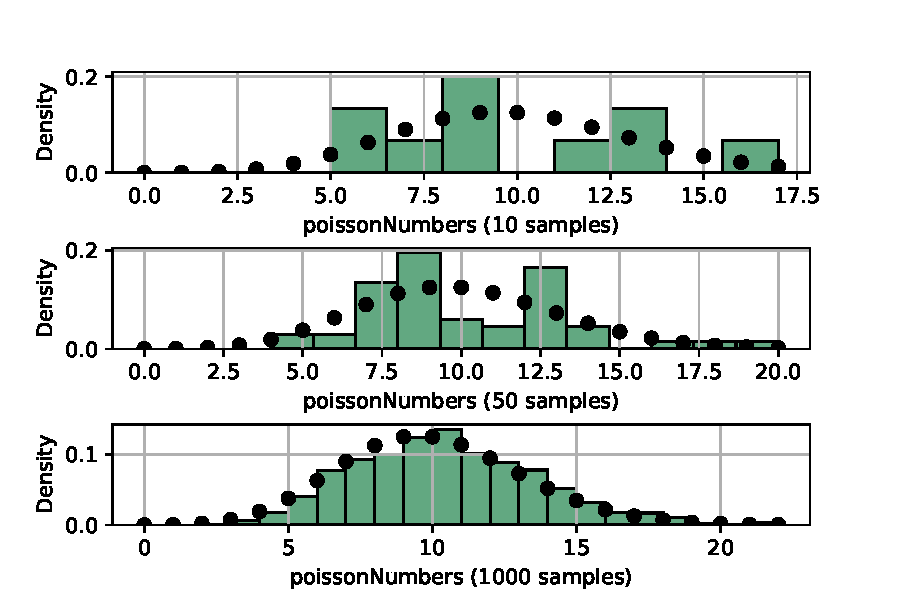
\includegraphics[width = 16 cm]{sources/poissonNumbers.pdf}
    \caption{Распределение Пуассона \eqref{poisson}}
    \label{fig:poisson}
\end{figure}
\begin{figure}[H]
    \centering
    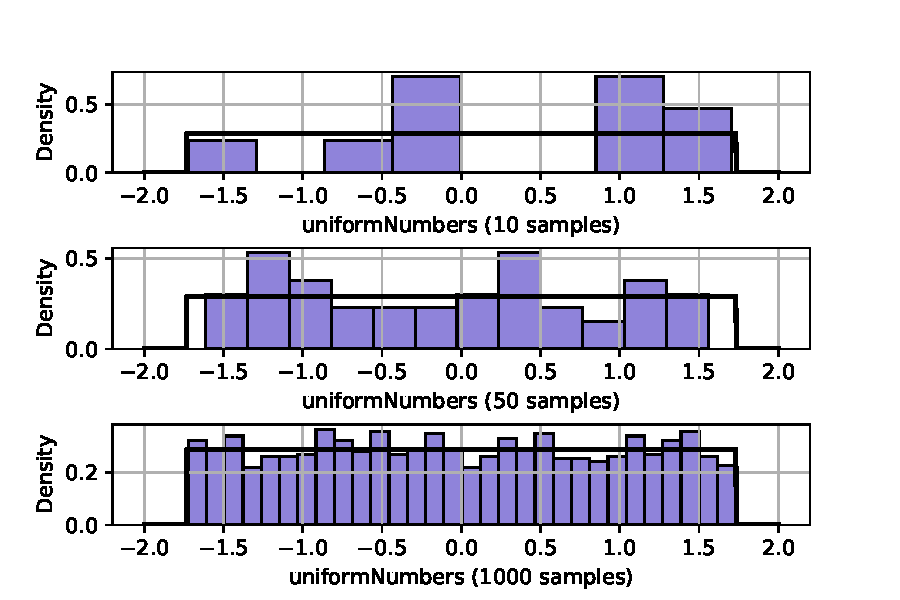
\includegraphics[width = 16 cm]{sources/uniformNumbers.pdf}
    \caption{Равномерное распределение \eqref{uniform}}
    \label{fig:uniform}
\end{figure}
\subsection{Характеристики положения и рассеивания}
\begin{table}[H]
    \centering
    \begin{tabular}{|c|c|c|c|c|c|}
        \hline
        normal $n$ = 10& & & & & \\
\hline
 &$\overline{x}\;\eqref{mean}$&$med\;x\;\eqref{med}$&$z_R\;\eqref{exhfsum}$&$z_Q\;\eqref{hfsum}$&$z_{tr}\;\eqref{trmean}$\\
\hline
$E(z)\;\eqref{mean_formula}$&0.001643&-0.001715&0.011264&0.307549&0.274457\\
\hline
$D(z)\;\eqref{variance_formula}$&0.105575&0.146178&0.174175&0.134176&0.123485\\
\hline
 & & & & & \\
\hline
normal $n$ = 100& & & & & \\
\hline
 &$\overline{x}$&$med\;x$&$z_R$&$z_Q$&$z_{tr}$\\
\hline
$E(z)$&-0.002837&-0.006377&0.010113&0.011054&0.021504\\
\hline
$D(z)$&0.010176&0.01538&0.09277&0.013052&0.012069\\
\hline
 & & & & & \\
\hline
normal $n$ = 1000& & & & & \\
\hline
 &$\overline{x}$&$med\;x$&$z_R$&$z_Q$&$z_{tr}$\\
\hline
$E(z)$&-0.002345&-0.001516&0.003679&-0.001195&0.000629\\
\hline
$D(z)$&0.001105&0.001723&0.063631&0.001349&0.001325\\
\hline

    \end{tabular}
    \caption{Нормальное распределение \eqref{norm}}
    \label{tab:norm}
\end{table}
\begin{table}[H]
    \centering
    \begin{tabular}{|c|c|c|c|c|c|}
        \hline
        cauchy $n$ = 10& & & & & \\
\hline
 &$\overline{x}$&$med\;x$&$z_R$&$z_Q$&$z_{tr}$\\
\hline
$E(z)$&4.032778&0.024677&19.86405&1.339201&0.776474\\
\hline
$D(z)$&10523.431164&0.337081&262430.774818&15.269762&2.615929\\
\hline
 & & & & & \\
\hline
cauchy $n$ = 100& & & & & \\
\hline
 &$\overline{x}$&$med\;x$&$z_R$&$z_Q$&$z_{tr}$\\
\hline
$E(z)$&-2.440452&-0.00389&-120.917099&0.037722&0.04242\\
\hline
$D(z)$&8567.668789&0.024353&21296287.803965&0.049615&0.02486\\
\hline
 & & & & & \\
\hline
cauchy $n$ = 1000& & & & & \\
\hline
 &$\overline{x}$&$med\;x$&$z_R$&$z_Q$&$z_{tr}$\\
\hline
$E(z)$&-1.639749&-0.001563&-846.555835&0.000551&0.001988\\
\hline
$D(z)$&952.311641&0.002561&235973354.703035&0.005211&0.002642\\
\hline

    \end{tabular}
    \caption{Распределение Коши \eqref{cauchy}}
    \label{tab:cauchy}
\end{table}
\begin{table}[H]
    \centering
    \begin{tabular}{|c|c|c|c|c|c|}
        \hline
        laplace $n$ = 10& & & & & \\
\hline
 &$\overline{x}$&$med\;x$&$z_R$&$z_Q$&$z_{tr}$\\
\hline
$E(z)$&-0.001668&-0.004131&0.010891&0.289294&0.226136\\
\hline
$D(z)$&0.101372&0.073895&0.401826&0.123031&0.085186\\
\hline
 & & & & & \\
\hline
laplace $n$ = 100& & & & & \\
\hline
 &$\overline{x}$&$med\;x$&$z_R$&$z_Q$&$z_{tr}$\\
\hline
$E(z)$&0.001346&-0.001301&0.028134&0.013016&0.019805\\
\hline
$D(z)$&0.010855&0.005921&0.421155&0.01084&0.006523\\
\hline
 & & & & & \\
\hline
laplace $n$ = 1000& & & & & \\
\hline
 &$\overline{x}$&$med\;x$&$z_R$&$z_Q$&$z_{tr}$\\
\hline
$E(z)$&-0.000328&-0.000592&-0.007745&0.00162&0.001773\\
\hline
$D(z)$&0.00091&0.000489&0.391542&0.0009&0.000573\\
\hline

    \end{tabular}
    \caption{Распределение Лапласа \eqref{laplace}}
    \label{tab:laplace}
\end{table}
\begin{table}[H]
    \centering
    \begin{tabular}{|c|c|c|c|c|c|}
        \hline
        poisson $n$ = 10& & & & & \\
\hline
 &$\overline{x}$&$med\;x$&$z_R$&$z_Q$&$z_{tr}$\\
\hline
$E(z)$&10.0383&9.8805&10.359&10.9795&10.811167\\
\hline
$D(z)$&0.952043&1.31197&1.984619&1.36983&1.170536\\
\hline
 & & & & & \\
\hline
poisson $n$ = 100& & & & & \\
\hline
 &$\overline{x}$&$med\;x$&$z_R$&$z_Q$&$z_{tr}$\\
\hline
$E(z)$&10.00143&9.848&10.9655&9.9655&9.94214\\
\hline
$D(z)$&0.098683&0.205396&0.97106&0.15006&0.117383\\
\hline
 & & & & & \\
\hline
poisson $n$ = 1000& & & & & \\
\hline
 &$\overline{x}$&$med\;x$&$z_R$&$z_Q$&$z_{tr}$\\
\hline
$E(z)$&9.997855&9.994&11.6445&9.9935&9.864184\\
\hline
$D(z)$&0.010238&0.005464&0.65537&0.003208&0.011762\\
\hline

    \end{tabular}
    \caption{Распределение Пуассона \eqref{poisson}}
    \label{tab:poisson}
\end{table}
\begin{table}[H]
    \centering
    \begin{tabular}{|c|c|c|c|c|c|}
        \hline
        uniform $n$ = 10& & & & & \\
\hline
 &$\overline{x}$&$med\;x$&$z_R$&$z_Q$&$z_{tr}$\\
\hline
$E(z)$&0.010428&0.007235&0.008858&0.333875&0.326122\\
\hline
$D(z)$&0.097559&0.218496&0.04188&0.126666&0.148893\\
\hline
 & & & & & \\
\hline
uniform $n$ = 100& & & & & \\
\hline
 &$\overline{x}$&$med\;x$&$z_R$&$z_Q$&$z_{tr}$\\
\hline
$E(z)$&-0.008995&-0.014935&-0.000303&0.007003&0.021455\\
\hline
$D(z)$&0.009266&0.026934&0.000616&0.014319&0.018513\\
\hline
 & & & & & \\
\hline
uniform $n$ = 1000& & & & & \\
\hline
 &$\overline{x}$&$med\;x$&$z_R$&$z_Q$&$z_{tr}$\\
\hline
$E(z)$&-0.000227&-0.000275&-3.3e-05&0.001693&0.003161\\
\hline
$D(z)$&0.001045&0.003089&6e-06&0.001582&0.002111\\
\hline

    \end{tabular}
    \caption{Равномерное распределение \eqref{uniform}}
    \label{tab:uniform}
\end{table}
\section{Обсуждение}
\subsection{Гистограмма и график плотности распределения}
Результаты проделанной работы указывают на то, что для каждого из распределений справедливо следующее замечание: при увеличении количества элементов выборки ее гистограмма становится ближе к графику плотности вероятности того закона, по которому распределены эти элементы. Чем меньше выборка, тем менее она репрезентативна и тем хуже по ней определяется характер распределения исследуемой величины.\\
\\
В большинстве случаев максимумы гистограмм и плотностей распределения не совпали. В некоторых местах прослеживаются всплески гистограмм, наиболее отчетливо - на распределении Коши.
\subsection{Характеристики положения и рассеяния}
В полученных данных, приведенных в таблице, особый интерес представляет дисперсия характеристик рассеяния для распределения Коши, чьи значения можно назвать аномально большими. Ясно, что это результат выбросов, которые можно было наблюдать в результатах предыдущего задания.
\section*{Примечание}
С кодом работы и отчета можно ознакомиться по ссылке:\;\url{https://github.com/Kozlov992/MS2021/tree/master/Labs1-2}
\end{document}
